\section{Probability and Information Theory}
\begin{multicols}{2}
	\subsection{Discrete Variables}
	\begin{itemize}
		\item Discrete \textbf{random variables} have a probability mass function (pmf) denoted by $P(x)$.
		\begin{itemize}
			\item Note that probability 0 is not impossible but \textbf{improbable}
			\item Also probability 1 is not certain just 100\% probable
		\end{itemize}
		\item The equation $ \sum_{x\in \bol{x}} P(x)=1$ must be satisfied
	\end{itemize}
	\textbf{Example:} A discrete RV with $k$ different states and uniform distribution.
	A uniform distribution means that every one of the $k$ states is equally likely, resulting in a pmf
	\[ P(\bol{x}=x_i)=\frac{1}{k} \]
	The notation $P(\bol{x}=x_i)$ means that this $P$ is the pmf of the RV $\bol{x}$ and we would like to evaluate it at state/value $x_i$.
	
	\subsection{Continuous Variables and pdfs}
	Since continuous RVs can take on an infinite number of values on the real number line, we cannot work with pmf.
	We therefore work with the \textbf{probability density function} (pdf).
	$p(x)$ is called the \textbf{likelihood}, not probability.\\
	
	The probability of $x$ being in an interval $\left[a,b\right]$ is
	\[ \int_a^b p(x)dx = 1 \]
	\textbf{Example:} An RV which is uniformly distributed on an interval $\left[a,b\right]$ of the real numbers.
	Within this interval $\left[a,b\right]$, $p(x)=\frac{1}{b-a}$, and outside of this interval, the function is zero.
	
	\subsection{Conditional Probability}
	One of the fundamental goals of machine learning is, that we would like to know the probability of one RV, given the knowledge about another one:
	\[ P(\bol{y}=y|\bol{x}=x)=\frac{P(\bol{y}=y,\bol{x}=x)}{P(\bol{x}=x)} \]
	
	Joint distributions over many RVs can be written as a product over conditional distributions, each being only over one variable:
	\[ P\left(x^{(1)},\dots,x^{(n)}\right) = P(x^{(1)}) \prod_{i=2}^{n} P\left( x^{(i)}|x^{(1)},\dots,x^{(i-1)} \right) \]
	For $n=3$:
	\begin{align*}
	P(a,b,c)
	&= P(a|b,c)P(b,c)\\
	&= P(a|b,c)P(b|c)P(c)
	\end{align*}
	
	\subsection{Expectation, Variance and Covariance}
	The ecpectation $\mu$ of a function $f()$ of a RV $x$ is the weighted average over the distribution $P(x)$:
	\begin{align*}
	\text{Discrete: }  &\Exp_{x\sim P}\left[f(x)\right] = \sum_x P(x)f(x)\\
	\text{Continuous: }  &\Exp_{x\sim p}\left[f(x)\right] = \int p(x)f(x)dx
	\end{align*}
	
	The expectation operator $\Exp$ is a linear operator:
	\[ \Exp_x \left[ \alpha f(x) + \beta g(x) \right] = \alpha\Exp_x \left[f(x)\right] + \beta\Exp_x \left[g(x)\right]\]
	
	The variance $\sigma^2$ measures the expected squared distance of $f(x)$ to its expected value $\Exp\left[f(x)\right]$:
	\begin{align*}
	\var\left( f(x) \right) &= \Exp \left[ \left( f(x) - \Exp \left[ f(x) \right] \right)^2 \right]\\
	&= \Exp \left[ f(x)^2 \right] - \Exp \left[ f(x) \right]^2
	\end{align*}
	For discrete RVs, the variance can be computed with
	\[ \var(X) = \sum_{i=1}^{n} p_i \cdot (x_i-\mu)^2 \]
	If they are all equally likely (uniformly distributed), this equation can be written as
	\[ \var(X) = \frac{1}{n} \sum_{i=1}^{n} (x_i-\mu )^2 \]
	
	The \textbf{covariance} gives some sense of how much two RVs are linearly related to each other and also the scale of these RVs:
	\[ \cov\left( f(x),g(y) \right) = 
	\Exp \left[ \left( f(x) -\Exp \left[ f(x) \right] \right)\left( g(y) -\Exp \left[ g(y) \right] \right) \right] \]
	
	The \textbf{correlation} is the covariance divided by the standard deviations $\sigma$ of $f(x)$ and $g(y)$ and can only be in the range of $–1$ to $+1$.\\
	
	The covariance matrix of a random vector $\bol{x}\in \mathbb{R}^n$ is an $n\times n$ matrix, such that
	\[ \cov(\bol{x})_{i,j}=\cov(x_i,x_j) \]
	The diagonal elements of the covariance matrix give the variance:
	\[ \cov(x_i,x_i) = \var(x_i) \]
	
	\subsection{Bernoulli Distribution}
	Fundamental distribution for a discrete RV that has only two states, usually called $0$ and $1$.
	It has a single parameter $\phi$, which is simply the probability of state $1$.
	\begin{align*}
	P(x=1) &= \phi \\
	P(x=0) &= 1-\phi\\
	P(\bol{x}=x) &= \phi^x(1-\phi)^{1-x}\\
	\Exp_x\left[x\right] &= \phi\\
	\var_x(x) &= \phi(1-\phi)
	\end{align*}
	
	\subsection{Multinoulli Distribution}
	A distribution over a discrete variable with $k$ different states.
	The parameter is a vector $\bol{p} \in \left[0,1\right]^{k-1}$ (with $k-1$ elements), where each entry $p_i$ is the probability of state $i$.
	The finale states probability $p_k$ is given by $1-\bol{1}^T\bol{p}$.
	Multinoulliis most often used to describe probabilities over a finite number of classes.
	
	\subsection{Gaussian Distribution}
	Most commonly used distribution over continuous RVs.
	\[ \mathcal{N}(x;\mu,\sigma^2) = \sqrt{\frac{1}{2\pi\sigma^2}}\exp\left(-\frac{1}{2\sigma^2}(x-\mu)^2\right) \]
	
	Multidimensional Gaussian distribution, where $\Sigma$ is the covariance matrix:
	\[ \mathcal{N}(\bol{x}; \bol{\mu},\bol{\Sigma}) = 
	\sqrt{\frac{1}{(2\pi)^n\det(\bol{\Sigma})}} 
	\exp \left( -\frac{1}{2} (\bol{x}-\bol{\mu})^T\bol{\Sigma}^{-1}(\bol{x}-\bol{\mu}) \right) \]
	
	\begin{itemize}
		\item For simplicity the covariance matrix is often assumed to be a diagonal matrix, hence all dimensions of $\bol{x}$ are uncorrelated.
		\item An even simpler model is the isotropic Gaussian distribution since the covariance matrix is simply a scalar times the identity matrix. Hence, the dimensions are not only uncorrelated but also all have the same variance.
	\end{itemize}
	
	\subsection{Exponential Distribution}
	\[ p(x;\lambda) = \lambda \bol{1}_{x\ge 0} \exp(-\lambda x) \]
	The $\bol{1}_{x\ge 0}()$ function is equal to the unit step, 1 for $x\ge 0$, 0 else.
	
	\subsection{Laplace Distribution}
	\[ \text{Laplace}(x;\mu,\gamma)=\frac{1}{2\gamma}\exp\left( -\frac{\lvert x-\mu \rvert }{\gamma} \right) \]
	The bigger $\gamma$, the steeper the peak at position $\mu$.
	
	\subsection{Useful Properties of Common Functions}
	\textbf{Logistic Sigmoid Function:}
	\begin{align*}
	\sigma(z) &= \frac{1}{1+e^{-z}}\\
	\sigma'(z)&= \sigma(z)\left[ 1-\sigma(z) \right]\\
	1-\sigma(z) &= \sigma(-z)
	\end{align*}
	
	\textbf{Softmax Function:}
	\begin{align*}
	\text{softmax}(\bol{x})_i = \frac{e^{x_i}}{\sum_{j=1}^{n}e^{x_j}}
	\end{align*}
	
	\textbf{Hyperbolic Tangent:}
	\begin{align*}
	h(z) &= \tanh(z)\\
	h'(z)&= 1-\left[h(z)\right]^2
	\end{align*}
	
	\textbf{Rectifier Linear Unit (ReLU):}
	\begin{align*}
	h(z) &= \max\left(0,z\right)\\
	h'(z)&= \begin{cases}
	1 & \text{if } z>0\\
	0 & \text{if } z\le 0
	\end{cases}
	\end{align*}
	
	\textbf{Softplus Function:}
	\begin{align*}
	\zeta(z) &= \log\left(1+\exp(x)\right)\\
	\zeta'(z)&= \sigma(z)\\
	-\zeta(-z) &= \log\left(\sigma(z)\right)\\
	\zeta(z) &= \int_{-\infty}^{x}\sigma(y)dy
	\end{align*}
	
	\subsection{Bayes' Rule}
	Bayes' rule is used to find $P(x|y)$ from $P(y|x)$ and $P(x)$. This is a common problem since the distribution of the measurements $y$ might be known for each state $x$. But to be able to decide which state to pick, we need the probability of that state $x$, given the particular measurement $y$.
	\begin{align*}
	P(x|y) &= \frac{P(x)P(y|x)}{P(y)}\\
	P(y)   &= \sum_x P(y|x)P(x)
	\end{align*}
	
	\subsection{Jacobian Matrix}
	\[ \bol{J} = 
	\begin{bmatrix} \frac{\partial \bol{f}}{\partial x_1} & \cdots & \frac{\partial \bol{f}}{\partial x_n} \end{bmatrix} = 
	\begin{bmatrix} 
	\frac{\partial f_1}{\partial x_1} & \cdots & \frac{\partial f_1}{\partial x_n}\\
	\vdots & \ddots & \vdots \\
	\frac{\partial f_m}{\partial x_1} & \cdots & \frac{\partial f_m}{\partial x_n}
	 \end{bmatrix}   \]
	
	\subsection{Information Theory}
	\begin{itemize}
		\item Likely events should have low information content
		\item Less likely events should have higher information content
		\item Independent events should have additive information
		\begin{itemize}
			\item For example, finding out that a tossed coin has come up as heads twice should convey twice as much information as finding out that a tossed coin has come up as heads once
		\end{itemize}
	\end{itemize}
	\[ I(x) = \log\left(\frac{1}{P(x)}\right) = -\log \left(P(x)\right) \]
	The average of this self-information describes the uncertainty of an entire distribution using the \textbf{Shannon entropy}:
	\[ H(x) = \Exp_{x\sim P}\left[I(x)\right] = -\Exp_{x\sim P}\left[\log P(x)\right] \]
	
	\begin{figure}[H]
		\centering
		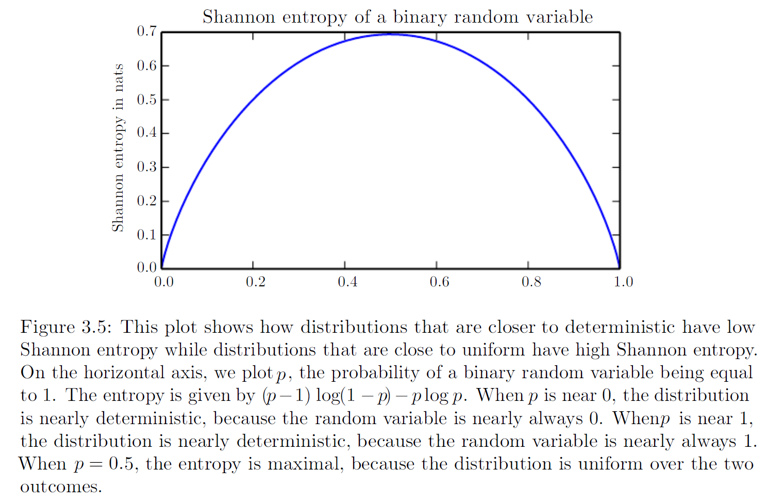
\includegraphics[width=1\linewidth]{images/shannon.png}
	\end{figure}

	\subsection{Kullback-Leibler Divergence}
	The KL divergence can be used to measure how different two distributions P and Q are:
	\[ D_{\text{KL}}(P\lVert Q) = \Exp_{x\sim P}\left[\log \frac{P(x)}{Q(x)}\right]=
	\Exp_{x\sim P}\left[\log {P(x)} \log {Q(x)}\right]
	 \]
	For discrete RVs this is the extra amount of information needed to send a message with symbols drawn from $P$, when the code was designed for $Q$.
	The \textbf{cross entropy} $H(P,Q)$ is the minimum average amount of information needed to transmit symbols drawn from $P(.)$ using a code designed for $Q(.)$:
	\[ H(P,Q) = -\sum_{x} P(x)\log \left(Q(x)\right) \]
	
	The entropy $H(P)$ is the minimum average amount of information needed to transmit symbols drawn from $P(.)$ using a code designed for $P(.)$:
	\[ H(P) = -\sum_{x} \log\left(P(x)\right) \]
	
	Hence the KL divergence is the difference DKL $(P\lVert Q)=H(P,Q)-H(P)$:
	\[ -\sum_{x} P(x)\log \left(Q(x)\right) +\sum_{x} \log\left(P(x)\right) \]
	
	The KL divergence is never negative, and zero if and only if $P$ and $Q$ are the same distributions.
	
\end{multicols}
\newpage













